%----------------------------------------------------------------
%
%  File    :  survey-animation.tex
%
%  Author  :  Keith Andrews, IICM, TU Graz, Austria
% 
%  Created :  27 May 1993
% 
%  Changed :  03 Feb 2017
% 
%----------------------------------------------------------------


\chapter{Animated Slideshow}

\label{chap:animated}

The biggest downside of the original \textit{rSlidy} when compared to alternative solutions, with focus on well spread desktop solutions, would be its static state. Namely the presentation flow achieved with the application was an immediate switch between states or slides. Even the user interface was behaving similarly in a state-switching way. In the design changes the effects of hiding elements with hover and transition CSS elements also include a better user experience. This follows the observations from the web animation survey \citet{WebAnime}, were the importance of animation for user experience was stressed out. With knowledge gathered from the mentioned survey we enhanced both the user interface as well the presentation flow by incorporating animation with CSS and JavaScript. For better overview, the animated old elements, that were already present in the original \textit{rSlidy}, have CSS added near the original class definitions, while the new concepts, sections \ref{sec:initialization} and \ref{sec:slide_transitions}, are defined in the new CSS file \textit{rslidy-animation.css}.

\section{Initialization Progress Animation} % (fold)
\label{sec:initialization}

\begin{figure}[tp]
	\centering
	
\includegraphics[width = .2\textwidth]{images/pulzLoad.png}
	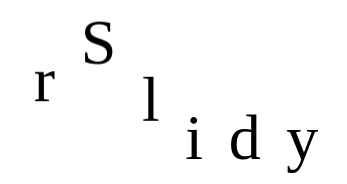
\includegraphics[width = .4\textwidth]{images/loading.png}	
	\caption[Loader]{
		Screenshot of the loading animations midway. On the left we see the inspirational pulz loader, while on the right we see the resulting rearrangement for \textit{rSlidy}.
		\imgcredit{Screenshot taken by the authors of this report.}
	}
	\label{fig:loading}
\end{figure}

% section initialization (end)

\section{Button Animation} % (fold)
\label{sec:button_animation}

Similar to an animated hamburger icon, which changes its shape on click, the buttons within the status bar of \textit{rSlidy} are animated now as well. Listing \ref{list:buttonflip} shows how the animated flip was created. These style changes and the button's text changed to an "X" lead to a simple and intuitive animation of a button which turns around to change its functionality. While the animation is done in CSS, the text change is done by the JavaScript setTimeout, to change the value halfway through the animation, when the text is not visible.
\begin{minipage}{\linewidth}
	\begin{lstlisting}[
	language=CSS,
	label=list:buttonflip,
	caption={[Flip Button Animation] Implementation of the animation of the buttons in the status bar %
	\imgcredit{The 
	code example is based 
	on the users' implementation.}
	}
	]
#button-overview, #button-toc, #button-menu{ 
	animation-duration: 0.3s; 
	animation-timing-function: ease-in-out;
	animation-fill-mode: forwards;
	animation-name: flip2Face;
}

#button-overview.clicked, #button-toc.clicked, #button-menu.clicked{
	animation-name: flip2Back; 
	transform: rotateY(180);
}
	\end{lstlisting}
\end{minipage}

\subsection{Same Element Animation Issue} % (fold)
\label{sub:same_element_animation_issue}

% subsection same_element_animation_issue (end)

% section button_animation (end)

\section{Hiding Elements} % (fold)
\label{sec:hiding_elements}

While hiding elements on hover elements by itself already raises the user experience, just by adding simple transition or animation CSS element we can direct the switch between states into a smooth way to enhance the user workflow. For better control we also used the Cubic Bezier function, with the values shown in figure \ref{fig:cubic-bezier}.

\begin{figure}[tp]
	\centering
	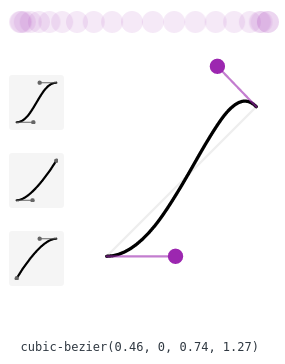
\includegraphics[width = .4\textwidth]{images/cubic-bezier.png}
	
	\caption[Cubic Bezier Function]{
		The values of the Cubic Bezier function used for smoother hiding of elements and its plot representation
		\imgcredit{Screenshot of the representation in Chrome Developer Tools taken by the authors of this report.}
	}
	\label{fig:cubic-bezier}
\end{figure}

% section hiding_elements (end)

\section{Preview Scrolling} % (fold)
\label{sec:preview_scrolling}

% section preview_scrolling (end)

\section{Slide Transitions} % (fold)
\label{sec:slide_transitions}

\subsection{Solution Limitations} % (fold)
\label{sub:solution_limitations}

% subsection solution_limitations (end)

\begin{figure}[tp]
	\centering
	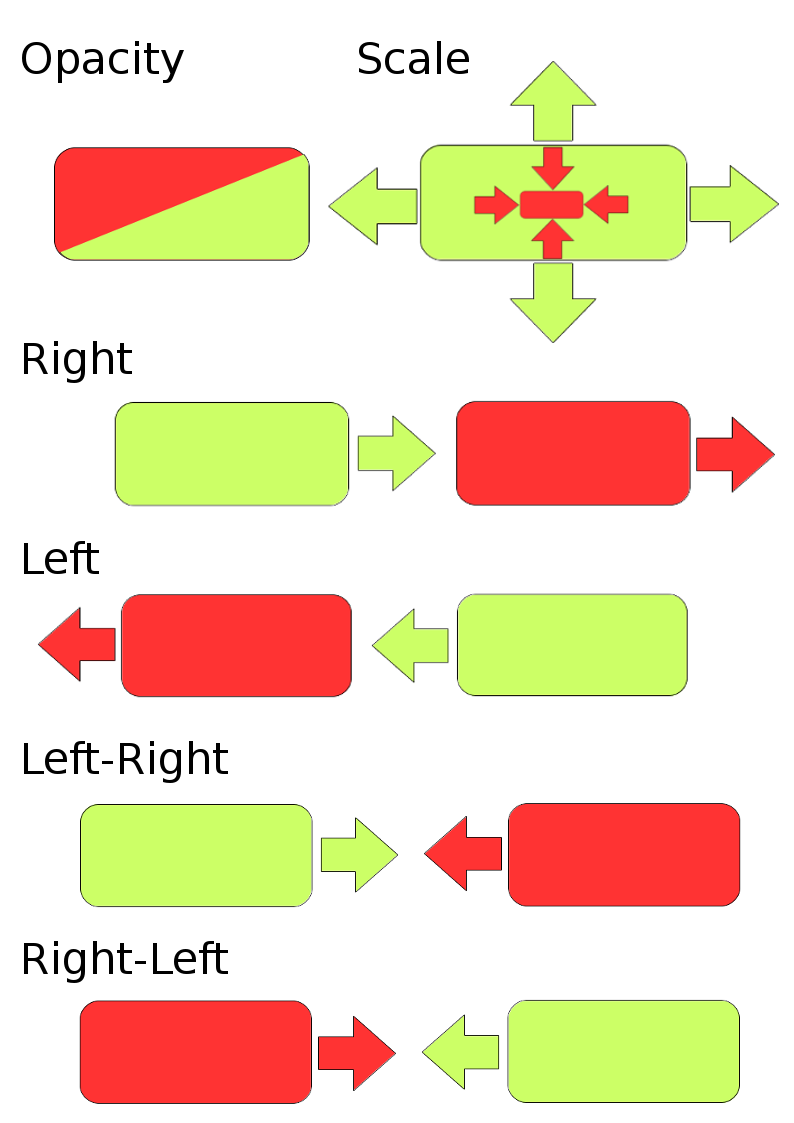
\includegraphics[width = .9\textwidth]{images/transitions.png}
	
	\caption[Slide Transition Diagram]{
		Diagram of \textit{rSlidy} included transitions and their flow. Red slides are the previous slides, while green are active slides. The position of active and previous slide is shown as relative position to the other.
		\imgcredit{Diagram is prepared by the authors of this report.}
	}
	\label{fig:transitions}
\end{figure}

% section slide_transitions (end)